\documentclass{article}
\usepackage[utf8]{inputenc}
\usepackage{graphicx}
\usepackage{amsmath}
\usepackage{ulem}
\usepackage{subfig}
\usepackage[margin=1.0in]{geometry}
\usepackage{caption}
\usepackage{subcaption}
\usepackage{wrapfig}
\usepackage{amsmath}
\usepackage{caption}
\usepackage{algorithm}
\usepackage[noend]{algpseudocode}
\usepackage{scrpage2}
\ifoot[]{}
\cfoot[]{}
\ofoot[\pagemark]{\pagemark}
\let\vec\mathbf

\title{Acceleration Structures}
\author{Ray Bai, Saketh Gabbita, Adapted from George Tang}
\date{February 12th, 2020}

\begin{document}

\maketitle

\section{Introduction}
Recall for rasterization, we discussed an optimization when for filling the triangle, we only search in the bounding box of the projection of the triangle. For raytracing, because each pixel's value is calculated by testing the ray associated with it against the scene objects, we can impose a partitioning scheme among the objects to accelerate the search process. The simplest scheme is to draw a bounding box around the object. We test all rays that intersect the box with the object (e.g. a teapot composed of hundreds of triangles); otherwise don't. Clearly, this will greatly accelerate the rendering process. This process is implemented through \textbf{acceleration structures}, data structures that support partitioning schemes.

\begin{figure}[!htbp]
 \centering
    \subfloat{{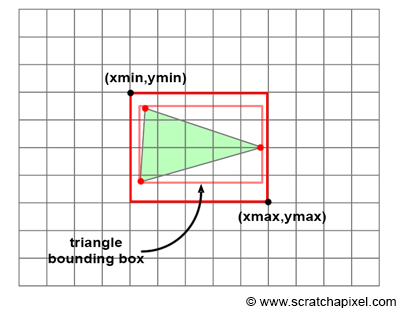
\includegraphics[width=6cm, height=4cm]{raster_bounding.png}}}%
    \qquad
    \subfloat{{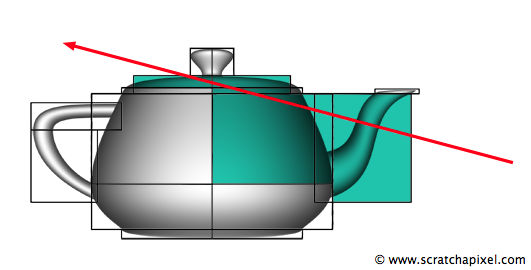
\includegraphics[width=6cm, height=4cm]{bb.png}}}%
    \caption{2D Bounding Boxes for Rasterization (left) vs. 3D Bounding Boxes for Raytracing (right)}%
    \label{fig:example}%
\end{figure}

\section{Ray-Box Intersection}
The simplest type of bounding box to deal with is the \textbf{axis aligned bounding box (AABB)}. As its name suggests, its sides are parallel to the x,y, z axis. For each bounding box we define $vmn$ and $vmx$, which are two diagonally opposite vertices, representing the least and greatest extent of the AABB from the perspective of the eye. 

A ray will have at most two intersection points with a finite box. If we extend the sides of the AABB infinitely, we will always have two intersections. Determining the distances to these intersections for the infinite AABB will allow us to determine if the ray intersects the definite AABB. We first only consider the case where there are no z bounding planes (x and y bounding planes extend infinitely).

again, our line can be defined parametrically and distance between the line and the lower x plane can we derived from

$$ \vec{O}.x+t_{mnx}\vec{d}.x = vmn.x $$
$$ t_{mnx} = \frac{(vmn.x-\vec{O}.x)}{\vec{d}.x}$$

And $t_{mxx}$, $t_{mny}$, and $t_{mxy}$ can be found using the same process.

\begin{figure}[!htbp]
 \centering
    \subfloat{{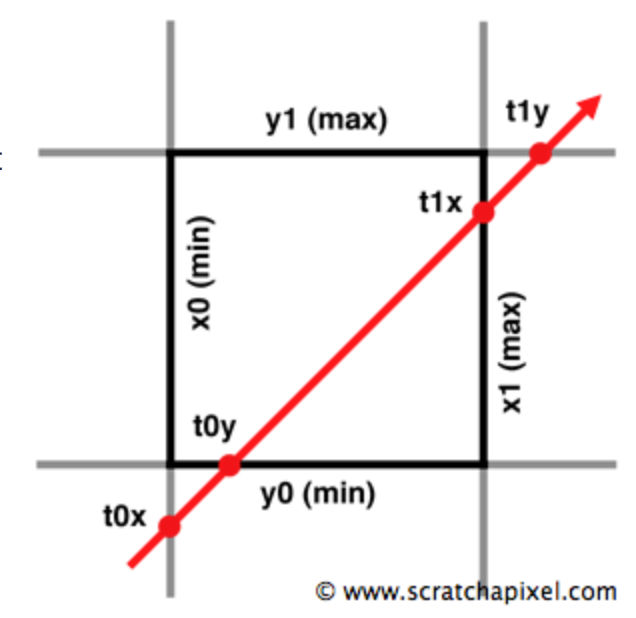
\includegraphics[width=7cm, height=6.5cm]{hit.png}}}%
    \qquad
    \subfloat{{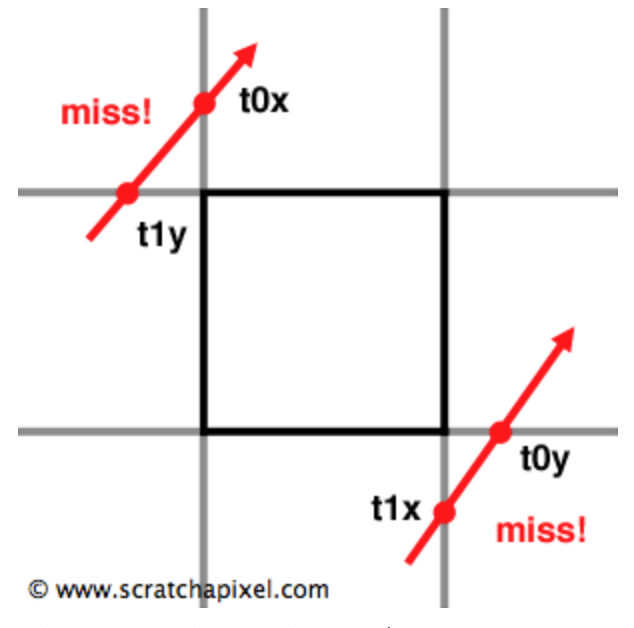
\includegraphics[width=7cm, height=6.5cm]{miss.png}}}%
    \caption{Hit case vs. Miss Case}%
    \label{fig:example}%
\end{figure}

We have two cases, illustrated in the diagram above. To test for the miss case, we test if $t_{mnx} > t_{mxy}$ or $t_{mny} > t_{mxx}$. We do the same for x and z bounding planes only. We have an intersection only if both x and y and x and z hit. A optimized implementation can be found at https://www.scratchapixel.com/lessons/3d-basic-rendering/minimal-ray-tracer-rendering-simple-shapes/ray-box-intersection.

\section{Bounding Volume Hierarchy}
Note if we have groups of individual volumes, we can group them and so forth. We can establish a hierarchy among the groups, known as a \textbf{Bounding Volume Hierarchy (BVH)}, further accelerating computation.

\begin{center}
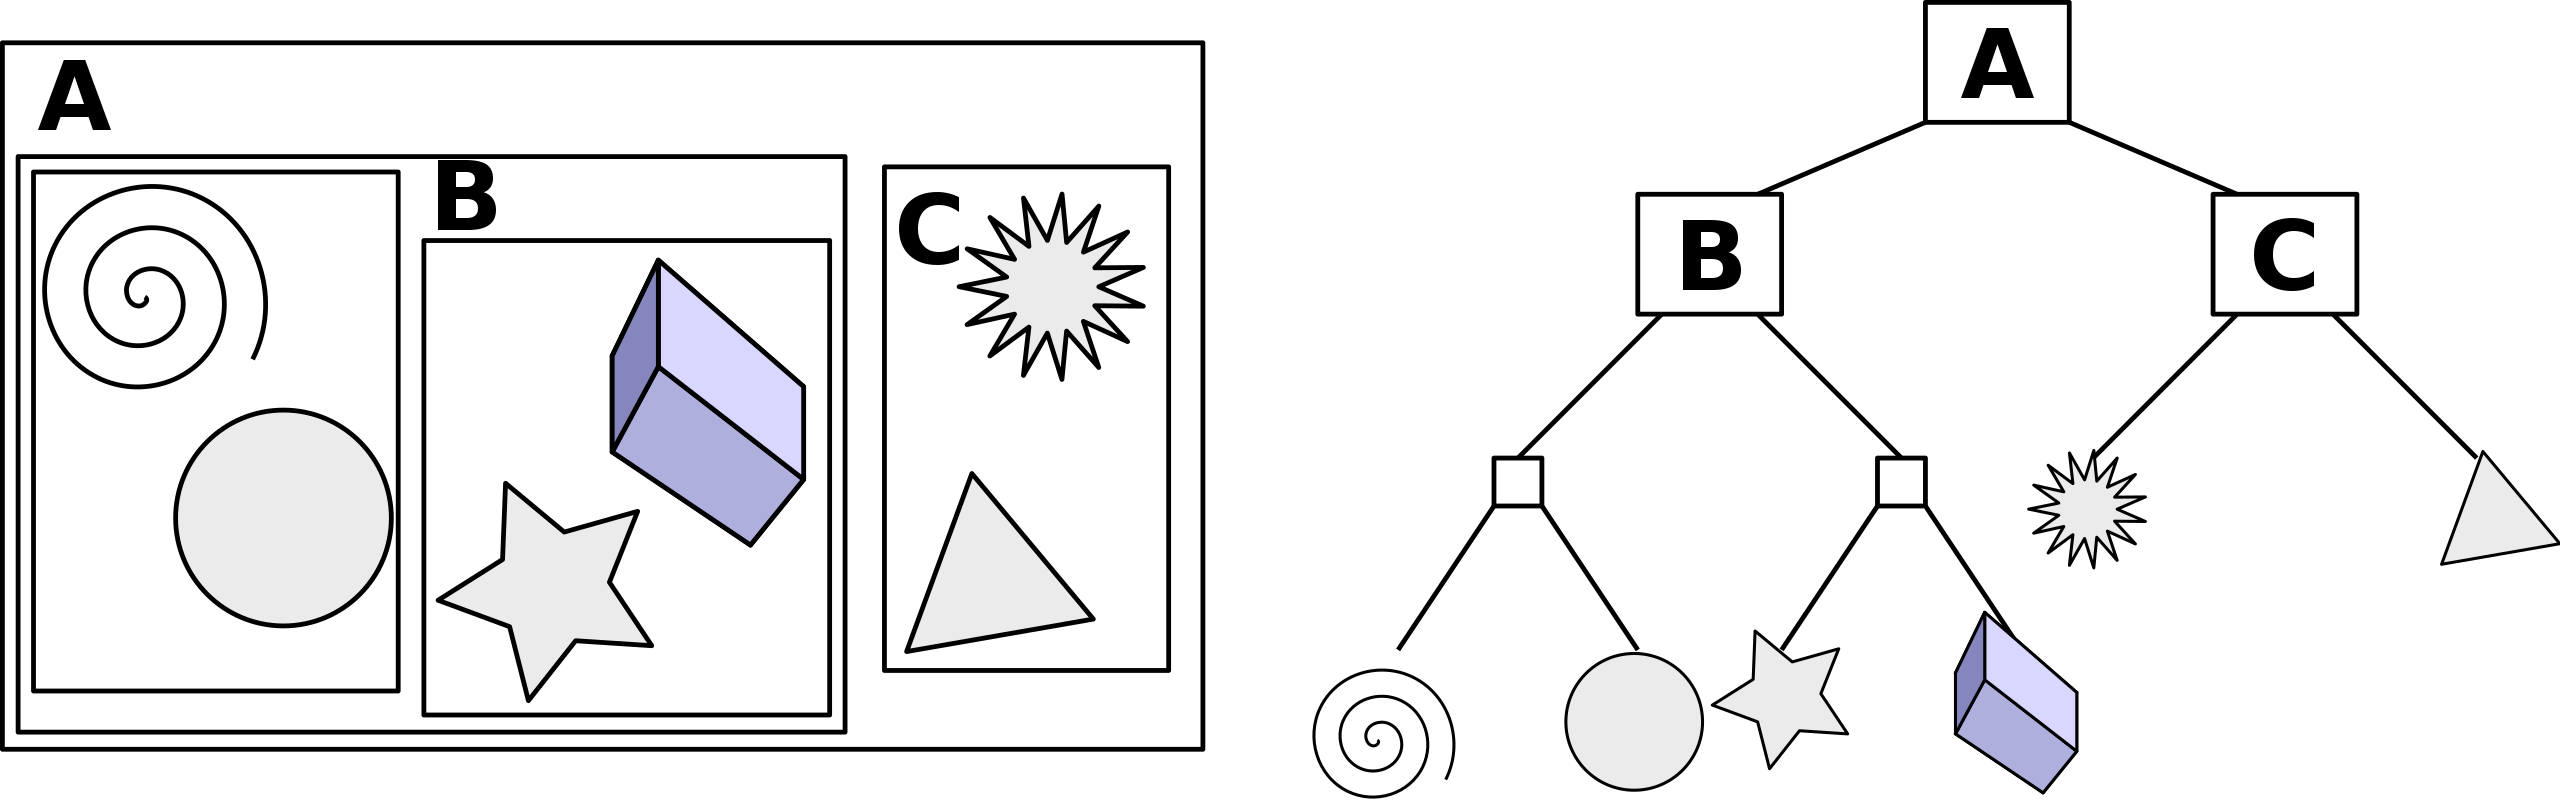
\includegraphics[width=14cm]{bvh.png}
\end{center}

\section{KD-Tree}
One way one the best BVHs (speed-wise and memory-wise) is the KD-Tree data structure. A KD-Tree consists of a build and a traversal algorithm. We begin with the root node encompassing all objects. Naive KD-build recursively assigns each object in a node to the left child or right child or both based on the object's location relative to the node's axis-aligned splitting plane. This plane is determined to be located at the median of the axis components of the triangles' centroids (represented as vectors). As we move down the tree during construction, we cycle through the x, y, z-axes and repeat. If the number of triangles is less than a certain threshold, then we stop splitting and denote the node as a leaf. Note only leaf nodes contain triangles. 

In the end, the axis-aligned splitting planes form bounding boxes that are used to determine if the ray intersects with any triangle in the group of triangles contained by the box. Because a KD-Tree divides the search space in two each time, the maximum depth is $log(N)$. Because we sort the triangles by axis component to determine the splitting plane when we construct each node, the overall time complexity for KD-build is $O(Nlog^2(N))$

\begin{figure*}[!h]
\begin{center}
  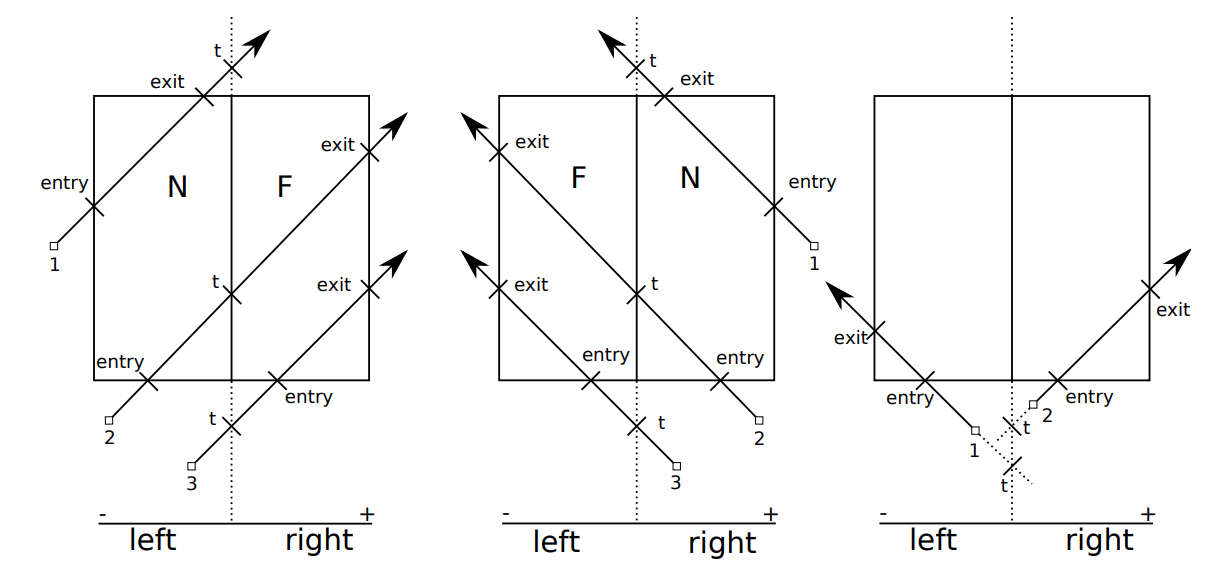
\includegraphics[width=15cm, height=6.5cm]{Casework.jpg}
  \caption{Casework for KD-traverse (see Algorithm 2). t refers the ray's distance to the splitting plane. If t is greater than the exit distance, then it only intersects the near node. If t is less, then it only intersects the far node. If t is in between, we have to search both nodes (from \cite{Hapala}).}
\end{center}
\end{figure*}

\begin{figure*}[h!]
\begin{minipage}[t]{3.35in}
\linespread{1.00}
\begin{algorithm}[H]
\caption{Naive KD-Build with SAH} 
\label{alg1} 
\begin{algorithmic}
    \Function{FindPlaneSAH}{$V$, $axis$}
        \State $best$ = none
        \State $minc$ = INF
        \For{$cent[axis]$ in $T$}
            \State $V_L, V_R \gets $Split$(cent[axis])$
            \State $curr$ = Cost($V_L$, $V_R$)
            \If{$ curr < minc$}
                \State $minc \gets curr$
                \State $best \gets cent[axis]$
            \EndIf
        \EndFor
        \State \Return $best$
    \EndFunction
    \vspace{0.05cm}
    \Function{KDBuild}{$V$, $depth$}
        \If {Terminate($V$)}
            \State \Return
        \EndIf
        \State $axis \gets depth$ \% 3
        \State $p \gets $FindPlaneSAH$(V, axis)$
        \State $V_L, V_R \gets $Split($p$)
        \State $T_L \gets \{t \in T \mid t \cap V_L \neq \emptyset\}$
        \State $T_R \gets \{t \in T \mid t \cap V_R \neq \emptyset\}$
        \State KDBuild($V_L$)
        \State KDBuild($V_R$)
    \EndFunction
\end{algorithmic}
\end{algorithm}
\end{minipage}
\hfill
\begin{minipage}[t]{3.35in}
\linespread{1.00}
\begin{algorithm}[H]
\caption{Naive KD-Traverse} 
\label{alg2} 
\begin{algorithmic}
    \Function{KDTraverse}{$V_{root}$, $ray$}
        \State $stack$.push($V_{root}$) 
        \While {$stack$ not empty}
            \State ($V$, $ent$, $ext$) $\gets$ $stack$.pop
            \While{$V$ not leaf}
                \State $t \gets$ DisToPlane$(V.p)$
                \State $V_{near}, V_{far} \gets $Classify$(V_L, V_R)$
                \If{$t \geq exit$ or $t<0$}
                    \State $V \gets V_{near}$
                    \State \textbf{continue}
                \EndIf
                \If{$t \leq ent$}
                    \State $V \gets V_{far}$
                \Else{}
                    \State $stack$.push($far$, $t$, $ext$)
                    \State $V \gets V_{near}$
                    \State $ext \gets t$
                \EndIf
            \EndWhile
            \If{FindIntersection($V$, $ray$)}
                \State \Return intersection
            \EndIf
        \EndWhile
        \State \Return $\emptyset$
    \EndFunction
\end{algorithmic}
\vspace{17pt}
\end{algorithm}
\end{minipage}
\hfill
\end{figure*}

The traversal algorithm is also recursive. Starting with the root node, we determine if the ray intersects it. If so, then we determine if it intersects only the left child, only the right child, or both, and traverse in accordance (Figure 2). If we reach a leaf node, we test intersection with every triangle in the node. The time complexity for KD-traverse is $O(log(N))$. 

One optimization we can make is instead of determining the splitting value based on the median of the axis component of the centroid, we locally maximize the probability that the ray will have to search fewer triangles. Intuitively, this translates to maximizing empty space in the bounding boxes, and formally we define the Surface Area Heuristic, which has been proven to be robust in almost all conditions.

The cost to traverse a node can be estimated given a splitting configuration, and we want to select the min cost configuration:

$$ Cost(V_L, V_R) \approx K_T + K_I\bigg(\frac{SA(V_L)}{SA(V)}T_L + \frac{SA(V_R)}{SA(V)}T_R \bigg) $$

where $V_L$, $V_R$, $V$ are the left, right, and parent voxels (nodes), $K_T$ is the cost of a bounding box intersection, $K_I$, the cost of a triangle intersection, $SA(V_L)$, $SA(V_R)$, $SA(V)$, the surface area of the left, right, and parent nodes, and $T_L$, $T_R$ the number of triangles in the left and right nodes.

\begin{figure}[!htbp]
 \centering
    \subfloat{{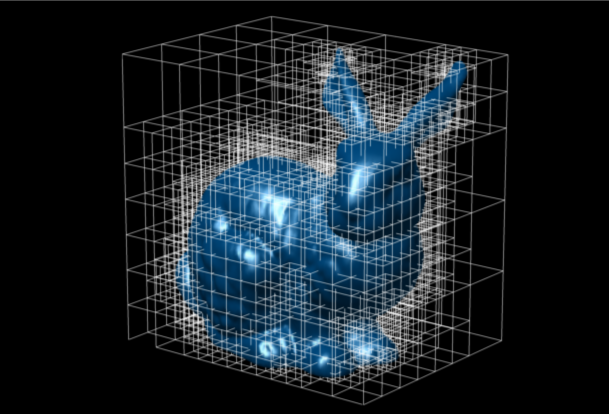
\includegraphics[width=7.5cm, height=6cm]{bunny.jpg}}}%
    \qquad
    \subfloat{{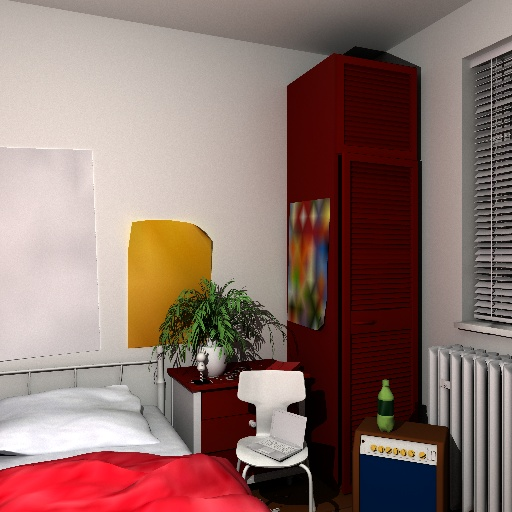
\includegraphics[width=6cm, height=6cm]{room149.jpg}}}%
    \caption{KD-Tree Partitioning of Stanford Bunny Model (left) and A Personal Rendering using KD-Tree (right)}%
    \label{fig:example}%
\end{figure}

\end{document}
